\cleardoublepage\chapter{Theoretical model}\label{chap:model}

\textsc{This is were we come} to the pith of the matter. A vehicle is made up of different magnetic materials. Some of them are soft magnetic materials\index{magnetic materials!soft magnetic material} and some are hard magnetic materials\index{magnetic materials!hard magnetic material}~\cite{imego2006}. The soft magnetic materials have no residual magnetisation but high magnetic susceptibility. The hard magnetic materials have high residual magnetisation. These materials all have the property that they will disturb a present magnetic field. The disturbances in a magnetic field created by a vehicle are large enough to be detected with a magnetic sensor.

Different vehicles will disturb a magnetic field differently due to the different magnetic materials and their distribution within the vehicle.

\section{The earth magnetic field}
The magnetic field\index{magnetic field} that we live and work in everyday is always changing. For this application it is of critical importance that the earth magnetic field\index{magnetic field!earth magnetic field} does not change too rapidly, at least not during the passing of a vehicle.

The magnetic field in a particular position has been known to be affected by magnetic mineral, iron artifacts, and similar. Short-term effects from solar flares are frequent. The earth magnetic field reverses polarity with an estimated frequency of a quarter of a million years. On a more rapid time scale, the field is estimated to have decayed about 5--15~\% over 150~years~\cite{nytimes}. Even if the decay is twice as much, it would not pose a problem for our application.

The earth magnetic field looks very different depending on your location in the world. The measurements discussed in this thesis have all been made in G\"{o}teborg, Sweden\footnote{Lat 57 43 00 N Long 011 58 00 E}. A common and non-complex model of the earth magnetic field can be seen in Figure~\ref{fig-earthmagnetic}.

\begin{figure}[!fbth]
 \centering
  \begin{minipage}{0.6\linewidth}
  \centering
   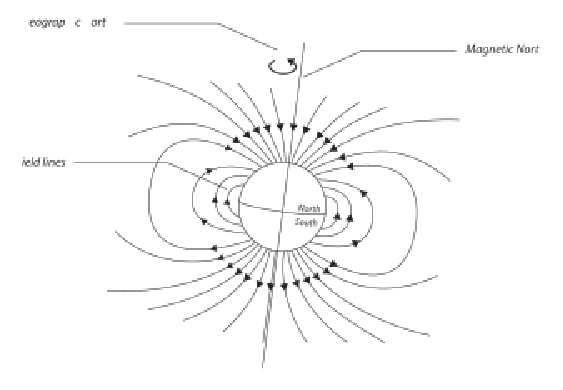
\includegraphics[width=1\linewidth]{images/earthmagnetic}
  \caption[Simplified model of the earth magnetic field]{Simplified model of the earth magnetic field. The earth magnetic field can be modelled like an ordinary magnet but in reality it is much more complex and is changing constantly.}
  \label{fig-earthmagnetic}
  \end{minipage}\hfill
\end{figure}

\section{Sensing the world}

The primary intent of a magnetic sensor is often not measuring the magnetic field. Instead one wishes to measure other parameters such as speed, heading, and presence, and to do so one has to look at the effect those parameters have on the magnetic field. Figures~\ref{fig:tradSensing} and~\ref{fig:magnSensing} illustrates the difference between conventional sensing\index{conventional sensing} and magnetic sensing\index{magnetic sensing}. In order to get the parameters we want from the magnetic fields, we have to apply signal processing.

\begin{subfigures}
\begin{figure}[!fbth]
 \centering\vfill
 \begin{minipage}{0.45\linewidth}\centering
      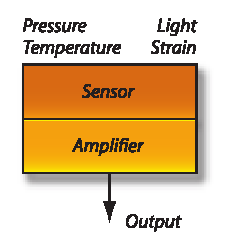
\includegraphics[width=.5\linewidth]{images/tradSensing}
 % sensoraxis.eps: 1179666x1179666 pixel, 300dpi, 9987.84x9987.84 cm, bb=
 \caption[Traditional sensing]{Conventional sensing.}
 \label{fig:tradSensing}
 \end{minipage}\hfill
 \begin{minipage}{0.45\linewidth}\centering
  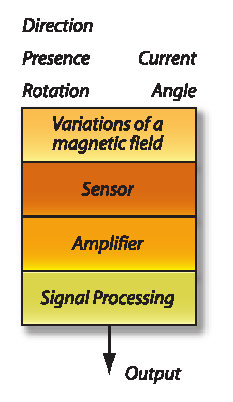
\includegraphics[width=.5\linewidth]{images/magnSensing}
 % sensoraxis.eps: 1179666x1179666 pixel, 300dpi, 9987.84x9987.84 cm, bb=
 \caption[Magnetic sensing]{Magnetic sensing\index{magnetic sensing}.}
 \label{fig:magnSensing}
 \end{minipage}
\end{figure}
\end{subfigures}

\section{Magnetic model}\index{magnetic model}

When a vehicle moves into a magnetic field the magnetic field lines are disturbed. These disturbances are not located solely inside the vehicle but also outside, allowing us to measure the magnetic field in order to sense the presence of that vehicle. See Figures~\ref{fig:before} and~\ref{fig:after}.
\begin{subfigures}
\begin{figure}[!th]
 \centering
 \begin{minipage}{0.45\linewidth}
 \centering
 	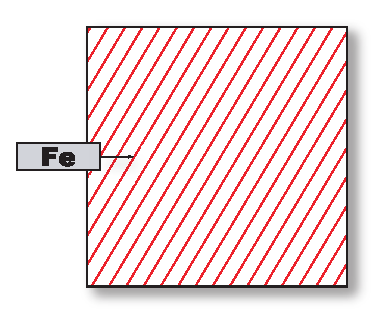
\includegraphics[height=5 cm]{images/before}
  	\caption[Non-disturbed field lines]{Non-disturbed field lines. A vehicle is about to enter.}
  	\label{fig:before} 
 \end{minipage} \hfill
 \begin{minipage}{0.45\linewidth}
 \centering
 	% generated by laprint.m
% %
% \begin{psfrags}%
% \psfragscanon%
%
% text strings:
\psfrag{s01}[b][b]{\fontsize{8}{12}\fontseries{m}\mathversion{normal}\fontshape{n}\selectfont \setlength{\tabcolsep}{0pt}\begin{tabular}{c}Passenger car\end{tabular}}%
\psfrag{s02}[t][t]{\fontsize{8}{12}\fontseries{m}\mathversion{normal}\fontshape{n}\selectfont \setlength{\tabcolsep}{0pt}\begin{tabular}{c}Time [s]\end{tabular}}%
\psfrag{s03}[b][b]{\fontsize{8}{12}\fontseries{m}\mathversion{normal}\fontshape{n}\selectfont \setlength{\tabcolsep}{0pt}\begin{tabular}{c}Magnetic field strength [nT]\end{tabular}}%
\psfrag{s06}[][]{\fontsize{10}{15}\fontseries{m}\mathversion{normal}\fontshape{n}\selectfont \setlength{\tabcolsep}{0pt}\begin{tabular}{c} \end{tabular}}%
\psfrag{s07}[][]{\fontsize{10}{15}\fontseries{m}\mathversion{normal}\fontshape{n}\selectfont \setlength{\tabcolsep}{0pt}\begin{tabular}{c} \end{tabular}}%
\psfrag{s08}[l][l]{\fontsize{6}{15}\fontseries{m}\mathversion{normal}\fontshape{n}\selectfont z}%
\psfrag{s09}[l][l]{\fontsize{6}{15}\fontseries{m}\mathversion{normal}\fontshape{n}\selectfont x}%
\psfrag{s10}[l][l]{\fontsize{6}{15}\fontseries{m}\mathversion{normal}\fontshape{n}\selectfont y}%
\psfrag{s11}[l][l]{\fontsize{6}{15}\fontseries{m}\mathversion{normal}\fontshape{n}\selectfont z}%
%
% axes font properties:
\fontsize{6}{15}\fontseries{m}\mathversion{normal}%
\fontshape{n}\selectfont%
%
% xticklabels:
\psfrag{x01}[t][t]{-0.2}%
\psfrag{x02}[t][t]{-0.1}%
\psfrag{x03}[t][t]{0}%
\psfrag{x04}[t][t]{0.1}%
\psfrag{x05}[t][t]{0.2}%
%
% yticklabels:
\psfrag{v01}[r][r]{-3000}%
\psfrag{v02}[r][r]{-2000}%
\psfrag{v03}[r][r]{-1000}%
\psfrag{v04}[r][r]{0}%
\psfrag{v05}[r][r]{1000}%
\psfrag{v06}[r][r]{2000}%
\psfrag{v07}[r][r]{3000}%
%
% Figure:
% \resizebox{6cm}{!}{\includegraphics{passengercar2.eps}}%
% \end{psfrags}%
% %
% End passengercar2.tex

  	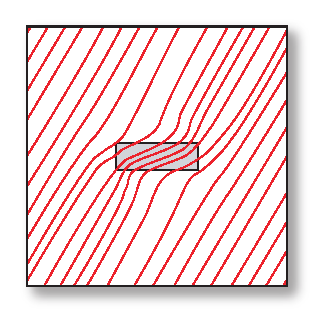
\includegraphics[height=5 cm]{images/after}
  	\caption[Field lines distributed by a vehicle]{Field lines distributed by a passing vehicle. Simulated in \textsc{Femlab}\footnotemark.}
  	\label{fig:after}
 \end{minipage}
  \end{figure}
 \end{subfigures}

% \begin{figure}
%  \centering
%  \begin{minipage}{0.6\linewidth}
%  \begin{asy}
import three;
import math;

size(6cm,0);

currentprojection=perspective(-15,10,10);

pair Sensor=(0,0,0);
pair r = (10,2,0);
pair Car=Sensor+r;

pair a=Car+(-1/2,-1/2,-1/2);
pair b=Car+(-1/2,1/2,-1/2);
pair c=Car+(1/2,1/2,-1/2);
pair d=Car+(1/2,-1/2,-1/2);

pair e=Car+(-1/2,-1/2,1/2);
pair f=Car+(-1/2,1/2,1/2);
pair g=Car+(1/2,1/2,1/2);
pair h=Car+1/2*(1,-1,1);


draw(a--b--c--d--(cycle));
draw(e--f--g--h--(cycle));

draw(a--e);
draw(b--f);
draw(c--g);
draw(d--h);

// velocity
//draw("$\vec{v}$",Car+(0,1,0)--Car+(0,2,0),Arrow);



// Axes

draw(Sensor--Sensor+(2,0,0),Arrow);
draw(Sensor--Sensor+(0,2,0),Arrow);
draw(Sensor--Sensor+(0,0,2),Arrow);
label("$\hat{x}'$",Sensor+(2,0,0),N);
label("$\hat{y}'$",Sensor+(0,2,0),N);
label("$\hat{z}'$",Sensor+(0,0,2),E);

draw(Car--Car+(2,0,0),Arrow);
draw(Car--Car+(0,2,0),Arrow);
draw(Car--Car+(0,0,2),Arrow);
label("$\hat{x}'$",Car+(2,0,0),N);
label("$\hat{y}'$",Car+(0,2,0),N);
label("$\hat{z}'$",Car+(0,0,2),E);

// position vector
draw("$\vec{r}$",Sensor--Car,Arrow);

pair a=Sensor+(-1/2,-1/2,-1/2);
pair b=Sensor+(-1/2,1/2,-1/2);
pair c=Sensor+(1/2,1/2,-1/2);
pair d=Sensor+(1/2,-1/2,-1/2);

pair e=Sensor+(-1/2,-1/2,1/2);
pair f=Sensor+(-1/2,1/2,1/2);
pair g=Sensor+(1/2,1/2,1/2);
pair h=Sensor+(1/2,-1/2,1/2);

draw(a--b--c--d--(cycle));
draw(e--f--g--h--(cycle));

draw(a--e);
draw(b--f);
draw(c--g);
draw(d--h);
//dot(unitcube,red);

label("Sensor",(0,0,0),E);



//road

draw((8,-10,0)--(8,10,0));
draw((11,-10,0)--(11,10,0));
\end{asy}

%  \caption{test!}
%  \end{minipage}
% \end{figure}x

All electromagnetics are governed by Maxwell's equations~\cite{cheng, feynman, Nordling:1995:PHS}\index{Maxwell's equations},

\begin{align}
	\nabla \cdot \vec{D} &= \rho_c & \text{Gauss's law}\index{Maxwell's equations!Gauss's law}\index{Gauss's law|see{Maxwell's equations}}\label{eq:gauss}\\
	\nabla \cdot \vec{B} &= 0 & \text{Gauss' law for magnetism}\index{Maxwell's equations!Gauss' law for magnetism}\index{Gauss' law for magnetism|see{Maxwell's equations}}\label{eq:gaussmag}\\
	\nabla \times \vec{E} &= -\frac{\partial\vec{B}}{\partial{}t} & \text{Faraday's law of induction}\index{Maxwell's equations!Faraday's law of induction}\index{Faraday's law of induction|see{Maxwell's equations}}\label{eq:faraday}\\
	\nabla \times \vec{H} &= \vec{J} + \frac{\partial{}\vec{D}}{\partial{}t} & \text{Amp\`{e}re's circuital law
	(with Maxwell's correction),}\index{Maxwell's equations!Amp\`{e}re's Circuital Law!with Maxwell's correction}\index{Amp\`{e}re's Circuital Law@amperes circuital|see{Maxwell's equations}}\label{eq:ampere}
\end{align}
where $\vec{B}$ is the magnetic flux density, $\vec{H}$ is the magnetic field strength, $\vec{E}$ is the electric flux density, $\vec{D}$ is the displacement field, $\vec{J}$ is the current density and \mbox{$\mu_0 =  4\pi \cdot 10^{-7}$ Vs/Am} is the permeability\index{permeability in vacuum} in vacuum~\cite{Nordling:1995:PHS}. $\mu_r$ is the relative permeability of the medium and $\rho_c$ is the electric charge density. In linear materials
\begin{align}
	\vec{D} &= \varepsilon_0 \vec{E} + \vec{P} = (1 + \chi_e) \varepsilon_0 \vec{E}
= \varepsilon \vec{E},\\
	\vec{B} &= \mu_0 (\vec{H} + \vec{M}) = (1 + \chi_m) \mu_0 \vec{H} = \mu_0\mu_r \vec{H},
\end{align}
where $\vec{P}$ is the polarisation density, $\vec{M}$ is the magnetisation density, $\chi_e$ is the electrical susceptibility and $\chi_m$ is the magnetic susceptibility. Assuming that the magnetic field is changing slowly, so that we reach a steady state, Maxwell's equations reduce~\cite{cheng, feynman, Nordling:1995:PHS} to the magnetostatic equations
\begin{align}
	\nabla \cdot \vec{B} &= 0 & \text{Gauss' law for magnetism\index{Maxwell's equations!Gauss' law for magnetism!magnetostatics}}\label{eq:gaussmagstat}\\
	\nabla \times \vec{B} &= \mu_0 \mu_r \vec{J} & \text{Amp\`{e}re's circuital law.\index{Maxwell's equations!Amp\`{e}re's Circuital Law!magnetostatics}}\label{eq:amperestat}
\end{align}
The vector potential of a magnetic dipole~\cite{Nordling:1995:PHS, feynman} can be written as
\begin{equation}
 \vec{A}(\vec{\mu},\vec{r}) = \frac{\mu_0}{4\pi}\frac{\vec{\mu}\times\vec{r}}{\left|\vec{r}\right|^3}, 
\end{equation}
where $\vec{\mu}$ is the magnetic moment and $\vec{r}$ is the vector from the dipole. This can be related to the magnetic flux density~\cite{Nordling:1995:PHS} by
\begin{equation}
	\vec{B} = \nabla \times \vec{A}.
\end{equation}
\footnotetext{Now \textsc{Comsol Multiphysics}, \url{http://www.comsol.com/}}%fulhack
The field from a magnetic dipole moment~\cite{imego2007}\index{magnetic dipole moment}\index{magnetic field!from a magnetic dipole moment} situated at the origin can then be written in vector form as
% \begin{equation}
%  \vec{B}(r,\theta) = \frac{\mu_0m}{4\pi{}r^3}\left(\hat{\vec{r}}\,2\cos{\theta} + \hat{\vec{\theta}}\,\sin{\theta}\right),\quad r,\theta \in \mathbb{R},
% \end{equation}
% where $m$ is the strength of the magnetic moment. The magnetic dipole is assumed to be oriented paralell to the $\hat{\vec{x}}$-axis. In vector form this becomes
\begin{equation}
 \vec{B}(\vec{\mu}_i,\vec{r}_i)=\frac{\mu_0}{4\pi} \frac{3\left(\vec{\mu}_i \cdot \vec{r}_i \right) \vec{r}_i - \vec{\mu}_i\left|\vec{r}_i\right|^2}{\left|\vec{r}_i\right|^5},\quad \vec{r}_i, \vec{\mu}_i \in \mathbb{R}^3.
\end{equation}

The total magnetic field, $\vec{B}$, from $n$ individual magnetic moments~\cite{imego2007} can be written as
\begin{align}
\vec{B}(\vec{r}_1,\vec{\mu}_1, \vec{r}_2, \vec{\mu}_2,...,\vec{r}_n,\vec{\mu}_n) &= \frac{\mu_0}{4\pi} \sum_{i=1}^{n} \frac{3\left(\vec{\mu}_i \cdot \vec{r}_i \right) \vec{r}_i - \vec{\mu}_i\left|\vec{r}_i\right|^2}{\left|\vec{r}_i\right|^5},
\end{align}
where $\vec{r}_i$ is the position for the $i$th magnetic moment $\vec{\mu}_i$.

It is assumed in~\cite{imego2007} that the permanent and induced magnetic fields from a vehicle\index{magnetic field!from a vehicle} can be viewed as the field from a number of magnetic moments. We shall later see that this is a good assumption. If we have knowledge of all the positions and strengths of the magnetic moments within the vehicle, we can calculate the field from that vehicle in any point in space. However, we will have an infinite number of magnetic moments.

Each of the magnetic moments will have six degrees of freedom, making a large system very complex to handle. Each vehicle will therefore be approximated to be comprised of a low number of magnetic moments.

The earth magnetic field\index{earth magnetic field} will have different direction and strength at different locations, but we can assume it to be constant near the sensor so that a vehicle will experience the same field in the vicinity of the sensor node. We also assume that the field does not change during the vehicle's passing of the sensor. The earth magnetic field does not have to be exactly equal at two different sensor node positions since the disturbances caused by the vehicle is similar. They are however not the same due to the orientation of the earth magnetic field and its impact on the magnetic dipole moments we assume our vehicle to be comprised of. For this application we assume that the magnetic dipoles are not time dependant. The time dependant magnetic field can now be written as
\begin{align}
\vec{B}(\vec{r}_1(t),\vec{\mu}_1, \vec{r}_2(t), \vec{\mu}_2,...,\vec{r}_n(t),\vec{\mu}_n) &= \frac{\mu_0}{4\pi} \sum_{i=1}^{n} \frac{3\left(\vec{\mu}_i \cdot \vec{r}_i(t) \right) \vec{r}_i(t) - \vec{\mu}_i\left|\vec{r}_i(t)\right|^2}{\left|\vec{r}_i(t)\right|^5}.
\end{align}

\begin{table}
\begin{minipage}{0.45\linewidth}
   \begin{center}
   \caption[Simulated magnetic field strength versus distance. Sensor in road surface.]{Maximum magnetic field strength at different distances from a passing passenger car. The node is placed in the road surface.}\vspace{2mm}
\label{tbl:strength1}
    \begin{tabular}{ c c }\toprule
      \textbf{Distance} [m] & $|B_z|$ [nT]\\ \midrule
% \rowcolor[gray]{.9}
      $0$ & $2.2 \cdot 10^5$ \\
      $1$ & $1765$ \\
% \rowcolor[gray]{.9}
      $2$ & $322$\\
      $3$ &$102$\\ \bottomrule
    \end{tabular}
  \end{center}
  \end{minipage}\hfill
  \begin{minipage}{0.45\linewidth}
      \begin{center}
   \caption[Simulated magnetic field strength versus distance. Sensor at 0.3 m.]{Maximum magnetic field strength at different distances from a passing passenger car. The node is placed at a height of 0.3 m.}
   \vspace{2mm}
\label{tbl:strength2}
    \begin{tabular}{cc}\toprule
      \textbf{Distance} [m] & $|B_z|$ [nT]\\ \midrule
% \rowcolor[gray]{.9}
      $0$ & $2.5 \cdot 10^{11}$ \\
      $1$ & $3000$ \\
% \rowcolor[gray]{.9}
      $2$ & $375$\\
      $3$ & $111$\\ \bottomrule
    \end{tabular}
  \end{center}
  \end{minipage}
\end{table}

\begin{figure}[htbf]
 \centering
 \begin{minipage}{0.6\linewidth}
 % generated by laprint.m
% %
% \begin{psfrags}%
% \psfragscanon%
%
% text strings:
\psfrag{s05}[b][b]{\fontsize{8}{12}\fontseries{m}\mathversion{normal}\fontshape{n}\selectfont \setlength{\tabcolsep}{0pt}\begin{tabular}{c}Magnetic field strength versus distance\end{tabular}}%
\psfrag{s06}[t][t]{\fontsize{8}{12}\fontseries{m}\mathversion{normal}\fontshape{n}\selectfont \setlength{\tabcolsep}{0pt}\begin{tabular}{c}Distance [m]\end{tabular}}%
\psfrag{s07}[b][b]{\fontsize{8}{12}\fontseries{m}\mathversion{normal}\fontshape{n}\selectfont \setlength{\tabcolsep}{0pt}\begin{tabular}{c}Magnetic field strength [nT]\end{tabular}}%
\psfrag{s10}[][]{\fontsize{10}{15}\fontseries{m}\mathversion{normal}\fontshape{n}\selectfont \setlength{\tabcolsep}{0pt}\begin{tabular}{c} \end{tabular}}%
\psfrag{s11}[][]{\fontsize{10}{15}\fontseries{m}\mathversion{normal}\fontshape{n}\selectfont \setlength{\tabcolsep}{0pt}\begin{tabular}{c} \end{tabular}}%
\psfrag{s12}[l][l]{\fontsize{8}{12}\fontseries{m}\mathversion{normal}\fontshape{n}\selectfont z}%
\psfrag{s13}[l][l]{\fontsize{8}{12}\fontseries{m}\mathversion{normal}\fontshape{n}\selectfont x}%
\psfrag{s14}[l][l]{\fontsize{8}{12}\fontseries{m}\mathversion{normal}\fontshape{n}\selectfont y}%
\psfrag{s15}[l][l]{\fontsize{8}{12}\fontseries{m}\mathversion{normal}\fontshape{n}\selectfont z}%
%
% axes font properties:
\fontsize{8}{12}\fontseries{m}\mathversion{normal}%
\fontshape{n}\selectfont%
%
% xticklabels:
\psfrag{x01}[t][t]{$0$}%
\psfrag{x02}[t][t]{$0.5$}%
\psfrag{x03}[t][t]{$1$}%
\psfrag{x04}[t][t]{$1.5$}%
\psfrag{x05}[t][t]{$2$}%
\psfrag{x06}[t][t]{$2.5$}%
\psfrag{x07}[t][t]{$3$}%
%
% yticklabels:
\psfrag{v01}[r][r]{$-2500$}%
\psfrag{v02}[r][r]{$-2000$}%
\psfrag{v03}[r][r]{$-1500$}%
\psfrag{v04}[r][r]{$-1000$}%
\psfrag{v05}[r][r]{$-500$}%
\psfrag{v06}[r][r]{$0$}%
\psfrag{v07}[r][r]{$500$}%
\psfrag{v08}[r][r]{$1000$}%
\psfrag{v09}[r][r]{$1500$}%
\psfrag{v10}[r][r]{$2000$}%
%
% Figure:
% \resizebox{6cm}{!}{\includegraphics{distance.eps}}%
% \end{psfrags}%
% %
% End distance.tex

 \includegraphics[width=1\linewidth]{images/distance}
 % placeholder.eps: 1179666x1179666 pixel, 300dpi, 9987.84x9987.84 cm, bb=
 \caption[Simulated magnetic field strength depending on distance]{Magnetic field strength depending on distance. The sensor is placed on the road surface and the field is measured exactly when the vehicle passes the sensor. This is not the point where the field is the strongest.}
 \label{fig:distance}
 \end{minipage}
\end{figure}

\section{Vehicle model}
In the model used, a vehicle of any type is said to be equivalent to at most three magnetic moments distributed in the car seen in \mbox{Figure \ref{fig:sensoraxis}}. A few simplifications are hereby made. The moments are assumed to be placed on the centerline of the vehicle, thereby reducing the degrees of freedom per magnetic moment by two. Since we have three magnetic moments each now having four degrees of freedom, we have a total number of twelve degrees of freedom. Compare this to the eighteen we had originally or even the unlimited degrees of freedom we really have. This is certainly a limitation of the model. The vehicle will move in a coordinate system relative to the sensor, where the sensor is placed in the origin.

The simulated maximum sfield strengths from a single passenger vehicle pass versus distance to sensor can be seen in Tables~\ref{tbl:strength1} and \ref{tbl:strength2} The simulated maximum field strengths versus distance at the instant the vehicle passes the sensor can be seen in Figure~\ref{fig:distance}.

\begin{figure}[!htbf]
 \centering
 \begin{minipage}{0.4\linewidth}
 \psfrag{x}{$\hat{x}$}
 \psfrag{y}{$\hat{y}$}
 \psfrag{z}{$\hat{z}$}
 \psfrag{r}{$\vec{r}$}
 \psfrag{v}{$v$}
 \psfrag{u1}{$\vec{\mu}_1$}
 \psfrag{u2}{$\vec{\mu}_2$}
 \psfrag{u3}{$\vec{\mu}_3$}
  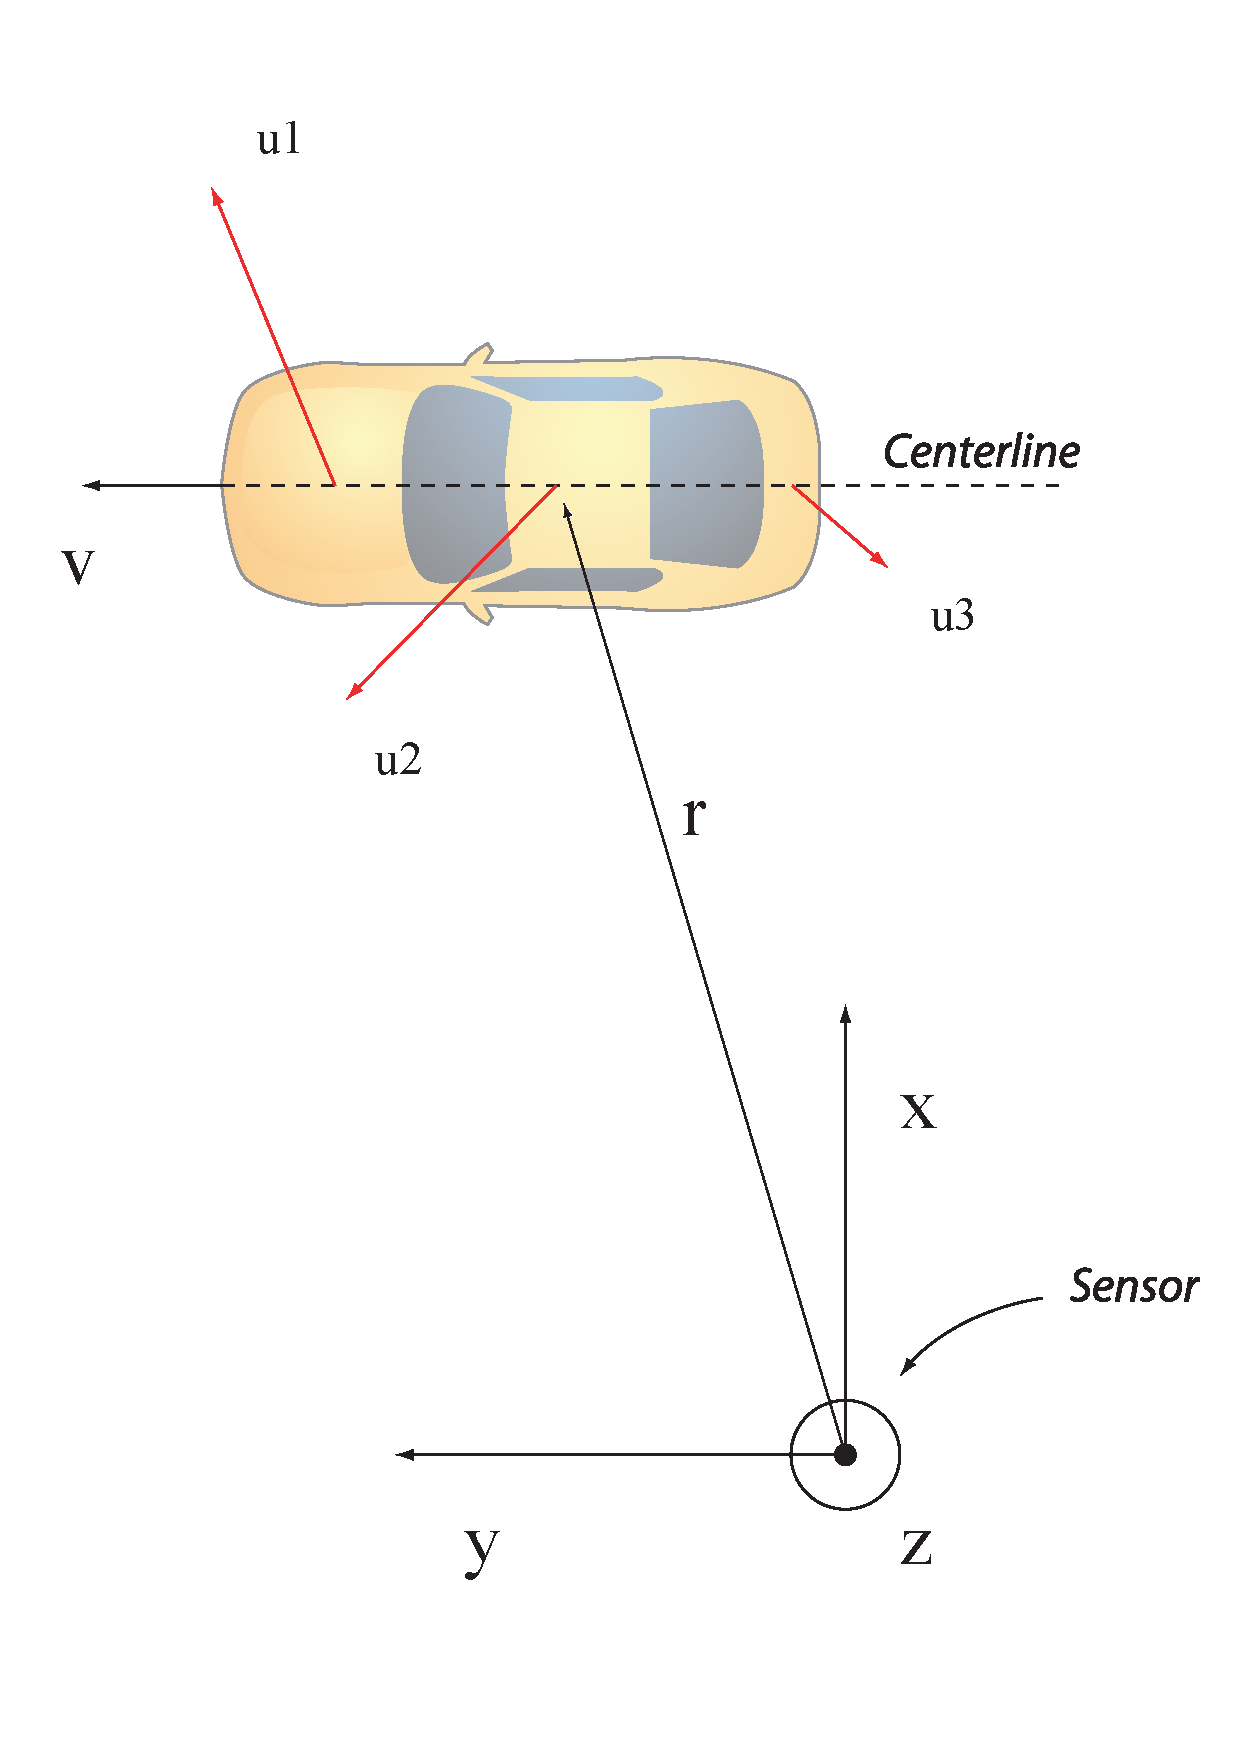
\includegraphics[width=1\linewidth]{images/sensoraxis}
 % sensoraxis.eps: 1179666x1179666 pixel, 300dpi, 9987.84x9987.84 cm, bb=
 \caption[Input parameters to the \textsc{Matlab}-model.]{Input parameters to the \textsc{Matlab}-model. The sensor is placed at the origin. The magnetic dipoles are assumed to be positioned on the vehicle centerline.}
 \label{fig:sensoraxis}
 \end{minipage}
\end{figure}

\section{Sensor and channel model}
\begin{figure}
	\centering
	\begin{minipage}{0.6\linewidth}
		\centering
		\psfrag{x}{$\hat{x}$}
		\psfrag{y}{$\hat{y}$}
		\psfrag{z}{$\hat{z}$}
		\psfrag{v}{$v$}
		\psfrag{u1}{$\vec{\mu}_1$}
		\psfrag{u2}{$\vec{\mu}_2$}
		\psfrag{u3}{$\vec{\mu}_3$}
		 \psfrag{ns(t)}{$\eta_{\sigma}(t)$}
		\includegraphics[width=1\linewidth]{images/channelmodel.eps}
		% channelmodel.eps: 1179666x1179666 pixel, 300dpi, 9987.84x9987.84 cm, bb=
		\caption{Can our channel be modelled as an AWGN channel?}
		\label{fig:channelmodel}
	\end{minipage}
\end{figure}

It is assumed that the data is affected by additive white Gaussian noise with some power as can be seen in Figure~\ref{fig:channelmodel}. We do not know exactly what the channel will do to the magnetic field, and we do not know exactly what the sensor will introduce, but their joint effect is modelled as an Additive White Gaussian Noise, AWGN, channel. The signal in one of the sensor axis is then represented by
\begin{equation}
x_i(\vec{r}_1(t),\vec{\mu}_1, \vec{r}_2(t), \vec{\mu}_2,...,\vec{r}_n(t),\vec{\mu}_n) = B_i(\vec{r}_1(t),\vec{\mu}_1, \vec{r}_2(t), \vec{\mu}_2,...,\vec{r}_n(t),\vec{\mu}_n) + \eta_{i,\sigma}(t),
\end{equation}
where $\eta_{i,\sigma}(t)$ is a zero-mean Gaussian distributed random variable with standard deviation $\sigma$ in direction $i \in \left\lbrace\hat{x}, \hat{y}, \hat{z}\right\rbrace$.

\subsection{Reconstruction}

As will be shown later we have sampled the signal at more than twice the Nyquist frequency\index{Nyquist frequency} and our signal $x(t)$ with one-sided baseband bandwidth $W$ is therefore uniquely determined by its samples
\begin{equation}
 x[n] = x(nT_s)\quad  n=0,\pm1, \ldots
\end{equation}
if the sampling frequency is
\begin{equation}
 f_s = \frac{1}{T_s} > 2W
\end{equation}
where the Fourier transform $X(f)$ of $x(t)$ satisfies 
\begin{equation}
X(f)=0\quad |f|>W. 
\end{equation}

$2W$ is called the Nyquist rate, and $f_s/2$ is the Nyquist frequency. We can now reconstruct the signal $x(t)$ by lowpass filtering~\cite{ali} the train of impulses \mbox{$x(nT_s)\delta{}(t-nT_s)$.} This will give us the reconstruction as
\begin{equation}
 x(t) = \sum_{n=-\infty}^{\infty} x(nT_s) \frac{\sin{\left(\pi{}(t-nT_s)/T_s\right)}}{\pi{}(t-nT_s)/T_s}.
\end{equation}

\section{Comparison to real world data} % Here?
Simulated data from four different vehicles can be seen in \mbox{Figures \ref{fig:simclass1}} \mbox{through \ref{fig:simclass4}}. The sensor has been placed \mbox{$1.5$ m} from the vehicles on the left side on the road surface. The speed was \mbox{100 km/h.} No noise was added. For the passenger car, one dipole situated 0.3~m over the sensor in the $\hat{z}$-direction and 0.7~m from the sensor in the $\hat{x}$-direction. The magnetic dipole strength was $[-3,0,-30]\,\text{Am}^2$, i.e., almost entirely in the negative $\hat{z}$-direction as expected at this location.

A comparison between simulated and real data for all axes can be found in Figures~\ref{fig:realdata} and~\ref{fig:simdata}. There are some discrepancies due to the fact that there are many unknown parameters in the measured data, such as velocity and distance to the sensor and these had to be estimated before simulation.

From this simple comparison we can conclude that our model is a reasonable model. However, we can not say anything about how good it is from this case where numerous parameters are unknown.

\begin{subfigures}
\begin{figure}[tfhb]
 \centering
 \begin{minipage}{0.45\linewidth}
 	\centering
 	% generated by laprint.m
%
% \begin{psfrags}%
% \psfragscanon%
%
% text strings:
\psfrag{s05}[b][b]{\fontsize{8}{12}\fontseries{m}\mathversion{normal}\fontshape{n}\selectfont \setlength{\tabcolsep}{0pt}\begin{tabular}{c}Passenger car\end{tabular}}%
\psfrag{s06}[t][t]{\fontsize{8}{12}\fontseries{m}\mathversion{normal}\fontshape{n}\selectfont \setlength{\tabcolsep}{0pt}\begin{tabular}{c}Time [s]\end{tabular}}%
\psfrag{s07}[b][b]{\fontsize{8}{12}\fontseries{m}\mathversion{normal}\fontshape{n}\selectfont \setlength{\tabcolsep}{0pt}\begin{tabular}{c}Magnetic field strength [nT]\end{tabular}}%
\psfrag{s10}[][]{\fontsize{10}{15}\fontseries{m}\mathversion{normal}\fontshape{n}\selectfont \setlength{\tabcolsep}{0pt}\begin{tabular}{c} \end{tabular}}%
\psfrag{s11}[][]{\fontsize{10}{15}\fontseries{m}\mathversion{normal}\fontshape{n}\selectfont \setlength{\tabcolsep}{0pt}\begin{tabular}{c} \end{tabular}}%
\psfrag{s12}[l][l]{\fontsize{6}{15}\fontseries{m}\mathversion{normal}\fontshape{n}\selectfont z}%
\psfrag{s13}[l][l]{\fontsize{6}{15}\fontseries{m}\mathversion{normal}\fontshape{n}\selectfont z}%
\psfrag{s14}[l][l]{\fontsize{6}{15}\fontseries{m}\mathversion{normal}\fontshape{n}\selectfont y}%
\psfrag{s15}[l][l]{\fontsize{6}{15}\fontseries{m}\mathversion{normal}\fontshape{n}\selectfont z}%
%
% axes font properties:
\fontsize{6}{15}\fontseries{m}\mathversion{normal}%
\fontshape{n}\selectfont%
%
% xticklabels:
\psfrag{x01}[t][t]{-0.2}%
\psfrag{x02}[t][t]{-0.1}%
\psfrag{x03}[t][t]{0}%
\psfrag{x04}[t][t]{0.1}%
\psfrag{x05}[t][t]{0.2}%
%
% yticklabels:
\psfrag{v01}[r][r]{-3000}%
\psfrag{v02}[r][r]{-2000}%
\psfrag{v03}[r][r]{-1000}%
\psfrag{v04}[r][r]{0}%
\psfrag{v05}[r][r]{1000}%
\psfrag{v06}[r][r]{2000}%
\psfrag{v07}[r][r]{3000}%
%
% Figure:
% \resizebox{6cm}{!}{\includegraphics{passengercar.eps}}%
% \end{psfrags}%
%
% End passengercar.tex

	\includegraphics[width=1\linewidth]{images/passengercar}
  	\caption[Simulated sensor data from passenger car]{Simulated sensor data from passenger car\index{magnetic field!from a car}.}
  	\label{fig:simclass1} 
 \end{minipage} \hfill
 \begin{minipage}{0.45\linewidth}
 	\centering
 	% generated by laprint.m
% %
% \begin{psfrags}%
% \psfragscanon%
%
% text strings:
\psfrag{s01}[b][b]{\fontsize{8}{12}\fontseries{m}\mathversion{normal}\fontshape{n}\selectfont \setlength{\tabcolsep}{0pt}\begin{tabular}{c}Passenger car\end{tabular}}%
\psfrag{s02}[t][t]{\fontsize{8}{12}\fontseries{m}\mathversion{normal}\fontshape{n}\selectfont \setlength{\tabcolsep}{0pt}\begin{tabular}{c}Time [s]\end{tabular}}%
\psfrag{s03}[b][b]{\fontsize{8}{12}\fontseries{m}\mathversion{normal}\fontshape{n}\selectfont \setlength{\tabcolsep}{0pt}\begin{tabular}{c}Magnetic field strength [nT]\end{tabular}}%
\psfrag{s06}[][]{\fontsize{10}{15}\fontseries{m}\mathversion{normal}\fontshape{n}\selectfont \setlength{\tabcolsep}{0pt}\begin{tabular}{c} \end{tabular}}%
\psfrag{s07}[][]{\fontsize{10}{15}\fontseries{m}\mathversion{normal}\fontshape{n}\selectfont \setlength{\tabcolsep}{0pt}\begin{tabular}{c} \end{tabular}}%
\psfrag{s08}[l][l]{\fontsize{6}{15}\fontseries{m}\mathversion{normal}\fontshape{n}\selectfont z}%
\psfrag{s09}[l][l]{\fontsize{6}{15}\fontseries{m}\mathversion{normal}\fontshape{n}\selectfont x}%
\psfrag{s10}[l][l]{\fontsize{6}{15}\fontseries{m}\mathversion{normal}\fontshape{n}\selectfont y}%
\psfrag{s11}[l][l]{\fontsize{6}{15}\fontseries{m}\mathversion{normal}\fontshape{n}\selectfont z}%
%
% axes font properties:
\fontsize{6}{15}\fontseries{m}\mathversion{normal}%
\fontshape{n}\selectfont%
%
% xticklabels:
\psfrag{x01}[t][t]{-0.2}%
\psfrag{x02}[t][t]{-0.1}%
\psfrag{x03}[t][t]{0}%
\psfrag{x04}[t][t]{0.1}%
\psfrag{x05}[t][t]{0.2}%
%
% yticklabels:
\psfrag{v01}[r][r]{-3000}%
\psfrag{v02}[r][r]{-2000}%
\psfrag{v03}[r][r]{-1000}%
\psfrag{v04}[r][r]{0}%
\psfrag{v05}[r][r]{1000}%
\psfrag{v06}[r][r]{2000}%
\psfrag{v07}[r][r]{3000}%
%
% Figure:
% \resizebox{6cm}{!}{\includegraphics{passengercar2.eps}}%
% \end{psfrags}%
% %
% End passengercar2.tex

  	\includegraphics[width=1\linewidth]{images/passengercar2}
  	\caption[Simulated sensor data from another passenger car]{Simulated sensor data from another passenger car.}
  	\label{fig:simclass2}
 \end{minipage}
  
 \begin{minipage}{0.45\linewidth}
 	\centering
 	% generated by laprint.m
%
% \begin{psfrags}%
% \psfragscanon%
%
% text strings:
\psfrag{s05}[b][b]{\fontsize{8}{12}\fontseries{m}\mathversion{normal}\fontshape{n}\selectfont \setlength{\tabcolsep}{0pt}\begin{tabular}{c}Bus\end{tabular}}%
\psfrag{s06}[t][t]{\fontsize{8}{12}\fontseries{m}\mathversion{normal}\fontshape{n}\selectfont \setlength{\tabcolsep}{0pt}\begin{tabular}{c}Time [s]\end{tabular}}%
\psfrag{s07}[b][b]{\fontsize{8}{12}\fontseries{m}\mathversion{normal}\fontshape{n}\selectfont \setlength{\tabcolsep}{0pt}\begin{tabular}{c}Magnetic field strength [nT]\end{tabular}}%
\psfrag{s10}[][]{\fontsize{10}{15}\fontseries{m}\mathversion{normal}\fontshape{n}\selectfont \setlength{\tabcolsep}{0pt}\begin{tabular}{c} \end{tabular}}%
\psfrag{s11}[][]{\fontsize{10}{15}\fontseries{m}\mathversion{normal}\fontshape{n}\selectfont \setlength{\tabcolsep}{0pt}\begin{tabular}{c} \end{tabular}}%
\psfrag{s12}[l][l]{\fontsize{6}{15}\fontseries{m}\mathversion{normal}\fontshape{n}\selectfont z}%
\psfrag{s13}[l][l]{\fontsize{6}{15}\fontseries{m}\mathversion{normal}\fontshape{n}\selectfont x}%
\psfrag{s14}[l][l]{\fontsize{6}{15}\fontseries{m}\mathversion{normal}\fontshape{n}\selectfont y}%
\psfrag{s15}[l][l]{\fontsize{6}{15}\fontseries{m}\mathversion{normal}\fontshape{n}\selectfont z}%
%
% axes font properties:
\fontsize{6}{15}\fontseries{m}\mathversion{normal}%
\fontshape{n}\selectfont%
%
% xticklabels:
\psfrag{x01}[t][t]{$-0.2$}%
\psfrag{x02}[t][t]{$-0.15$}%
\psfrag{x03}[t][t]{$-0.1$}%
\psfrag{x04}[t][t]{$-0.05$}%
\psfrag{x05}[t][t]{$0$}%
\psfrag{x06}[t][t]{$0.05$}%
\psfrag{x07}[t][t]{$0.1$}%
\psfrag{x08}[t][t]{$0.15$}%
\psfrag{x09}[t][t]{$0.2$}%
%
% yticklabels:
\psfrag{v01}[r][r]{$-1$}%
\psfrag{v02}[r][r]{$-0.5$}%
\psfrag{v03}[r][r]{$0$}%
\psfrag{v04}[r][r]{$0.5$}%
\psfrag{v05}[r][r]{$1$}%
\psfrag{ypower}[Bl][Bl]{$\times 10^{4}$}%
%
% % Figure:
% \resizebox{6cm}{!}{\includegraphics{bus.eps}}%
% \end{psfrags}%
%
% End bus.tex

    	\includegraphics[width=1\linewidth]{images/bus}
  	\caption[Simulated sensor data from a bus]{Simulated sensor data from bus\index{magnetic field!from a bus}. Note the complexity.}
  	\label{fig:simclass3}
 \end{minipage} \hfill
 \begin{minipage}{0.45\linewidth}
 	\centering
 	\input{images/highcar.tex}
   	\includegraphics[width=1\linewidth]{images/highcar}
  	\caption[Simulated sensor data from high car]{Simulated sensor data from high car\index{magnetic field!from a high car}. Note the complexity.}
  	\label{fig:simclass4}
 \end{minipage}
\end{figure}
\end{subfigures}

\begin{subfigures}
\begin{figure}[tfhb]
 \centering
 \begin{minipage}{0.45\linewidth}
 	\centering
 	% generated by laprint.m
%
% \begin{psfrags}%
% \psfragscanon%
%
% text strings:
\psfrag{s05}[b][b]{\fontsize{8}{12}\fontseries{m}\mathversion{normal}\fontshape{n}\selectfont \setlength{\tabcolsep}{0pt}\begin{tabular}{c}Measurement data\end{tabular}}%
\psfrag{s06}[t][t]{\fontsize{8}{12}\fontseries{m}\mathversion{normal}\fontshape{n}\selectfont \setlength{\tabcolsep}{0pt}\begin{tabular}{c}Time [s]\end{tabular}}%
\psfrag{s07}[b][b]{\fontsize{8}{12}\fontseries{m}\mathversion{normal}\fontshape{n}\selectfont \setlength{\tabcolsep}{0pt}\begin{tabular}{c}Magnetic field strength [nT]\end{tabular}}%
\psfrag{s10}[][]{\fontsize{8}{12}\fontseries{m}\mathversion{normal}\fontshape{n}\selectfont \setlength{\tabcolsep}{0pt}\begin{tabular}{c} \end{tabular}}%
\psfrag{s11}[][]{\fontsize{8}{12}\fontseries{m}\mathversion{normal}\fontshape{n}\selectfont \setlength{\tabcolsep}{0pt}\begin{tabular}{c} \end{tabular}}%
\psfrag{s12}[l][l]{\fontsize{6}{8}\fontseries{m}\mathversion{normal}\fontshape{n}\selectfont $\hat{z}$}%
\psfrag{s13}[l][l]{\fontsize{6}{8}\fontseries{m}\mathversion{normal}\fontshape{n}\selectfont $\hat{x}$}%
\psfrag{s14}[l][l]{\fontsize{6}{8}\fontseries{m}\mathversion{normal}\fontshape{n}\selectfont $\hat{y}$}%
\psfrag{s15}[l][l]{\fontsize{6}{8}\fontseries{m}\mathversion{normal}\fontshape{n}\selectfont $\hat{z}$}%
%
% axes font properties:
\fontsize{6}{8}\fontseries{m}\mathversion{normal}%
\fontshape{n}\selectfont%
%
% xticklabels:
\psfrag{x01}[t][t]{$73$}%
\psfrag{x02}[t][t]{$73.2$}%
\psfrag{x03}[t][t]{$73.4$}%
\psfrag{x04}[t][t]{$73.6$}%
\psfrag{x05}[t][t]{$73.8$}%
\psfrag{x06}[t][t]{$74$}%
\psfrag{x07}[t][t]{$74.2$}%
\psfrag{x08}[t][t]{$74.4$}%
\psfrag{x09}[t][t]{$74.6$}%
\psfrag{x10}[t][t]{$74.8$}%
%
% yticklabels:
\psfrag{v01}[r][r]{$-3000$}%
\psfrag{v02}[r][r]{$-2000$}%
\psfrag{v03}[r][r]{$-1000$}%
\psfrag{v04}[r][r]{$0$}%
\psfrag{v05}[r][r]{$1000$}%
\psfrag{v06}[r][r]{$2000$}%
\psfrag{v07}[r][r]{$3000$}%
\psfrag{v08}[r][r]{$4000$}%
\psfrag{v09}[r][r]{$5000$}%
\psfrag{v10}[r][r]{$6000$}%
%
% % Figure:
% \resizebox{6cm}{!}{\includegraphics{realdata.eps}}%
% \end{psfrags}%
%
% End realdata.tex

	\includegraphics[width=1\linewidth]{images/realdata}
  	\caption[Measured sensor data from passenger car]{Measured sensor data from passenger car~\cite{imego2007}. Note the different timescale due to difference in speed.\\}
  	\label{fig:realdata} 
 \end{minipage} \hfill
 \begin{minipage}{0.45\linewidth}
 	\centering
 	\input{images/simdata.tex}
  	\includegraphics[width=1\linewidth]{images/simdata}
  	\caption[Simulated sensor data from passenger car]{Simulated sensor data from passenger car. Speed was 30~km/h and the distance to the sensor was 0.7~m. The sensor was placed on the roadway.}
  	\label{fig:simdata}
 \end{minipage}
\end{figure}
\end{subfigures}
% \subsection{One magnetic moment}
% \begin{figure}
%  % text strings:
% \psfrag{s05}[t][t]{\color[rgb]{0,0,0}\setlength{\tabcolsep}{0pt}\begin{tabular}{c}Time [s]\end{tabular}}%
% \psfrag{s06}[b][b]{\color[rgb]{0,0,0}\setlength{\tabcolsep}{0pt}\begin{tabular}{c}Magnetic field [nT]\end{tabular}}%
% \psfrag{s10}[][]{\color[rgb]{0,0,0}\setlength{\tabcolsep}{0pt}\begin{tabular}{c} \end{tabular}}%
% \psfrag{s11}[][]{\color[rgb]{0,0,0}\setlength{\tabcolsep}{0pt}\begin{tabular}{c} \end{tabular}}%
% %
% % xticklabels:
% \psfrag{x01}[t][t]{-0.3}%
% \psfrag{x02}[t][t]{-0.2}%
% \psfrag{x03}[t][t]{-0.1}%
% \psfrag{x04}[t][t]{0}%
% \psfrag{x05}[t][t]{0.1}%
% \psfrag{x06}[t][t]{0.2}%
% \psfrag{x07}[t][t]{0.3}%
% %
% % yticklabels:
% \psfrag{v01}[r][r]{-150}%
% \psfrag{v02}[r][r]{-100}%
% \psfrag{v03}[r][r]{-50}%
% \psfrag{v04}[r][r]{0}%
% \psfrag{v05}[r][r]{50}%
% \psfrag{v06}[r][r]{100}%
% \psfrag{v07}[r][r]{150}%
% 
% \psfrag{s13}{$\hat{x}$-direction}
% \psfrag{s14}{$\hat{y}$-direction}
% \psfrag{s15}{$\hat{z}$-direction}
% 
% \psfrag{Magnetic Field Strength}{Magnetic Field Strength}
% \psfrag{Time}{Time}
% \centering
%   \begin{minipage}{0.6\linewidth}
%   \centering
%    \includegraphics[width=1\linewidth]{images/sim1}
%   \caption[Simulated magnetic field from passing magnetic moment.]{Simulated magnetic field from passing magnetic moment \mbox{$\mu_1 = 0.1\,\hat{x} -0.2 \,\hat{y} + 1 \,\hat{z}$} at a distance of $1$ m from the sensor and at a speed of $30$ km/h.}
%   \label{fig-sim1}
%   \end{minipage}\hfill
% \end{figure}



